\documentclass[aspectratio=169]{beamer}
\usepackage{fontspec}
\usefonttheme{professionalfonts}
\usepackage{amsmath,amssymb,amsthm}
\usepackage{arydshln,mathtools}
\usepackage{bm}
\usepackage{color}
\definecolor{theme}{RGB}{0,73,114}
\usepackage{multicol}
%\usepackage[caption=false]{subfig}
\usepackage{subcaption}

\usepackage{comment}

\usepackage{graphicx}
\usepackage{diffcoeff}
\usepackage{dsfont}
\usepackage{mathrsfs}
\usepackage[most]{tcolorbox}

\usepackage{xspace}
\usepackage{appendixnumberbeamer}


\usepackage{media9}
\usepackage[backend=bibtex, style=verbose]{biblatex}

\bibliography{biblio_DissDyn}
%\renewcommand\bibfont{\scriptsize}

\addtobeamertemplate{footnote}{\vspace{-6pt}\advance\hsize-0.5cm}{\vspace{6pt}}
\makeatletter
% Alternative A: footnote rule
\renewcommand*{\footnoterule}{\kern -3pt \hrule \@width 2in \kern 8.6pt}
% Alternative B: no footnote rule
% \renewcommand*{\footnoterule}{\kern 6pt}
\makeatother


\makeatletter
\g@addto@macro\normalsize{%
	\setlength\abovedisplayskip{4pt}
	\setlength\belowdisplayskip{4pt}
	\setlength\abovedisplayshortskip{4pt}
	\setlength\belowdisplayshortskip{4pt}
}
\makeatother

% Math macros
\DeclareMathOperator*{\grad}{grad}
\DeclareMathOperator*{\Grad}{Grad}
\DeclareMathOperator*{\Div}{Div}
\renewcommand{\div}{\operatorname{div}}
\DeclareMathOperator*{\Hess}{Hess}
\DeclareMathOperator*{\curl}{curl}
\DeclareMathOperator{\Tr}{Tr}
\DeclareMathOperator{\Dom}{Dom}
\DeclareMathOperator*{\esssup}{ess\,sup}

\newcommand{\bbR}{\mathbb{R}}
\newcommand{\bbC}{\mathbb{C}}
\newcommand{\bbF}{\mathbb{F}}
\newcommand{\bbA}{\mathbb{A}}
\newcommand{\bbB}{\mathbb{B}}
\newcommand{\bbS}{\mathbb{S}}

\newcommand*{\norm}[1]{\ensuremath{\left\|#1\right\|}}
\newcommand{\where}{\qquad \text{where} \qquad}
\newcommand{\inner}[3][]{\ensuremath{\left\langle #2, \, #3 \right\rangle_{#1}}}
\newcommand{\bilprod}[2]{\left\langle \left\langle \, #1, #2 \, \right\rangle \right\rangle}
\newcommand{\pder}[2]{\ensuremath{\partial_{#2} #1}}
\newcommand{\dder}[2]{\ensuremath{\delta_{#2} #1}}
\newcommand{\secref}[1]{\S\ref{#1}}
\newcommand{\energy}[1]{\frac{1}{2} \int_{\Omega} \left\{ #1 \right\} \d\Omega}
\newcommand{\crmat}[1]{\ensuremath{\left[#1\right]_\times}}
\newcommand{\fenics}{\textsc{FEniCS}\xspace}
\newcommand{\firedrake}{\textsc{Firedrake}\xspace}

\DeclareMathOperator*{\argmax}{arg\,max}
\DeclareMathOperator*{\argmin}{arg\,min}

\newtheorem{proposition}{Proposition}
\newtheorem{remark}{Remark}
\newtheorem{hypothesis}{Hypothesis}
\newtheorem{assumption}{Assumption}
\newtheorem{conjecture}{Conjecture}


\def\onedot{$\mathsurround0pt\ldotp$}
\def\cddot{% two dots stacked vertically
	\mathbin{\vcenter{\baselineskip.67ex
			\hbox{\onedot}\hbox{\onedot}}%
}}


\setbeamertemplate{blocks}[rounded][shadow]

\setbeamercolor{block body alerted}{bg=alerted text.fg!10}
\setbeamercolor{block title alerted}{bg=alerted text.fg!20}
\setbeamercolor{block body}{bg=structure!10}
\setbeamercolor{block title}{bg=structure!20}
\setbeamercolor{block body example}{bg=green!10}
\setbeamercolor{block title example}{bg=green!20}

% Remove navigation bar
\setbeamertemplate{navigation symbols}{}

\addtobeamertemplate{navigation symbols}{}{%
	\usebeamerfont{footline}%
	\usebeamercolor[fg]{footline}%
	\hspace{1em}%
	\insertframenumber/\inserttotalframenumber
}


\makeatletter \renewcommand\d[1]{\ensuremath{%
		\;\mathrm{d}#1\@ifnextchar\d{\!}{}}}
\makeatother


\graphicspath{{./imagesDiss/}}

\newif\iftocsub
\tocsubtrue
\AtBeginSection[] {
	\begin{frame}[noframenumbering]{Outline}
		\tableofcontents[sectionstyle=show/shaded, subsectionstyle=show/show/hide]
	\end{frame}
	\tocsubfalse
}
\AtBeginSubsection[] {
	\iftocsub
	\begin{frame}[noframenumbering]{Outline}
		\tableofcontents[currentsubsection, sectionstyle=show/shaded, subsectionstyle=show/shaded/hide]
	\end{frame}
	\fi
	\tocsubtrue
}

\newcommand{\beginbackup}{
	\newcounter{framenumbervorappendix}
	\setcounter{framenumbervorappendix}{\value{framenumber}}
}
\newcommand{\backupend}{
	\addtocounter{framenumbervorappendix}{-\value{framenumber}}
	\addtocounter{framenumber}{\value{framenumbervorappendix}} 
}


\begin{document}
	
	
\begin{frame}[plain]
	
	\input{TitleDissSys}
	
\end{frame}
	
	
\begin{frame}{Outline}
	
	\tableofcontents
	
\end{frame}

\section{Introduction}

\begin{frame}{Why dissipative dynamical systems?}

\begin{tcolorbox}[width=0.95\textwidth, nobeforeafter, colframe=theme,title=All engineering systems exhibit dissipation.]
\begin{itemize}
	\item Electrical networks with resistors;
	\item Mechanical systems (viscoelastic or Coulomb friction);
	\item Thermodynamic systems: dissipation leads to an increase in entropy.
\end{itemize}
\end{tcolorbox}
The notion of dissipativity establishes a natural link between the properties of input-output and state-space models. Many modern computational tools for the analysis and synthesis of control systems  are based on it.
\vspace{.3cm}

\footnotesize{
\fullcite{willems1972part1}\\
\fullcite{willems1972part2}\\
\cite{schaft1999l2}}

\end{frame}

\begin{frame}{Some mathematical notation}
$\bbR_+ = [0, \infty)$ denotes the set of positive reals. \\
$\bbR^2_+:=\{(t_1, t_2) \in \bbR^2 |\;  t_2\ge t_1\}$ (causal triangular sector of $\bbR^2$). \\
Let $V$ be a finite dimensional normed liner space with norm $||\cdot||_V$. \\
\vspace{.1cm}
(If $V=\bbR^n$ then the Euclidean norm is denoted by$||x||_2 = \sqrt{x^\top x}$)

\begin{definition}[Local $L^p_{\text{loc}}$ Banach spaces]
	For each positive integer $p \in {1, 2, \dots}$, the set $L^p_{\text{loc}}(\bbR, V)$ consists of all functions $f : \bbR \rightarrow V$, which are measurable and satisfy
	\begin{equation*}
		\int_a^b ||f(t)||^p_V \d t< \infty, \qquad \forall\,  a, b \in \bbR.
	\end{equation*}
	The case $p=\infty$ consists of all bounded measurable functions on compact intervals, i.e. $\sup_{t \in [a, b]} f(t) < \infty.$
	
\end{definition}

\end{frame}



\begin{comment}
	
	\begin{definition}[$L^p$ Banach spaces]
		For each positive integer $p \in {1, 2, \dots}$, the set $L^p(\bbR, V)$ consists of all functions $f : \bbR \rightarrow V$, which are measurable and satisfy
		\begin{equation*}
			\int_{\bbR} ||f(t)||^p_V \d t< \infty,
		\end{equation*}
		The case $p=\infty$ consists of all bounded measurable functions, i.e. $\sup_{t \in \bbR} f(t) < \infty.$
		The $L^p$ spaces are Banach spaces (complete normed linear spaces) w.r.t. the norm
		\begin{equation*}
			||f||_{L^p} = \left(\int_0^\infty ||f(t)||^p_V \d t \right)^{\frac{1}{p}}, \quad q=1,2,\dots \qquad ||f||_{L^\infty} = \sup_{t \in \bbR} |f(t)|, \quad q=\infty.
		\end{equation*} 
		
	\end{definition}
	
	\begin{definition}[Extended $L^p$ Banach spaces]
		For each $T \in \bbR_+$ the function $f_T: \bbR_+ \rightarrow V$ defined by
		\begin{equation*}
			f_T= 
			\begin{cases}
				f(t), \\
				0, 
			\end{cases} \quad
			\begin{aligned}
				0\le t < T, \\
				t \ge T
			\end{aligned}
		\end{equation*}
		is called the truncation of $f$.\\
		For $q=1,2,\dots, \infty$ the set $L^{pe}(\bbR_+, V)$ consists of all measurable functions $f: \bbR_+ \rightarrow V$ such that $f_T \in L^p(\bbR_+, V), \quad  \forall T, \; 0 \le T < \infty$. \\
		The spaces $L^{pe}$ are called the extended $L^p$ spaces. It holds $L^p(\bbR_+, V) \subset L^{pe}(\bbR_+, V)$.
	\end{definition}
	
\end{comment}

\begin{frame}{General setting}
Consider the state-space system  with inputs and outputs
\begin{equation*}
	\Sigma : \quad 
	\begin{aligned}
		\dot{x} &= f(x, u), \\
		y &= h(x,u),
	\end{aligned} \qquad
	\begin{aligned}
		u(t) \in U, \\
		y(t) \in Y,
	\end{aligned}
\end{equation*} 
where $x(t) \in \mathcal{X}$. In general $\mathcal{X}$ is a manifold and $U,\; Y$ vector spaces. \\

For sake simplicity, assume $\mathcal{X} \subseteq \bbR^n,\; U=\bbR^m, \; Y=\bbR^p$.

\begin{theorem}
	Suppose $f, h$ to be Lipschitz continuous in $x$ and $u$ jointly. \\
	Then system $\Sigma$ has a unique solution $\forall x(t_0) \in \mathcal{X}, \; u(\cdot) \in L^2_{\text{loc}}(\bbR, U)$ with $x(\cdot) \in L^2_{\text{loc}}(\bbR, \mathcal{X}), \ y(\cdot) \in L^2_{\text{loc}}(\bbR, Y)$.
\end{theorem}

\end{frame}

\begin{frame}{Reachability and controllability}
\begin{overlayarea}{\textwidth}{\textheight}
	
\begin{definition}[State transition function]
		Given the system $\Sigma$, the state transition function $\phi$ is the map 
		\begin{equation*}
			\phi(t_1, t_0, x(t_0), u(\cdot)) : \bbR_+^2 \times \mathcal{X} \times L^{2}_{\text{loc}}(\bbR, U) \rightarrow \bbR^n
		\end{equation*}
		such that $x(t_1) = \phi(t_1, t_0, x(t_0), u(\cdot))$. 
\end{definition}


\begin{definition}[Reachability and controllability]
		The state space $\mathcal{X}$ of system $\Sigma$ is said to be \textbf{reachable}
		from $x_{-1}$ if 
		\begin{equation*}
		\forall\, x \in \mathcal{X}, \; \exists\,  t_{-1} \le 0, \, \exists\, u(\cdot) \in L^{2}_{\text{loc}}(\bbR, U) \text{ such that } x = \phi(0, t_{-1}, x_{-1}, u(\cdot)).
		\end{equation*}
				It is said to be \textbf{controllable} to $x_1$ if 
		\begin{equation*}
			\forall\, x \in \mathcal{X}, \; \exists\, t_1 > 0, \; \exists \, u(\cdot) \in L^{2}_{\text{loc}}(\bbR, U) \text{ such that } x_1 = \phi(t_1, 0, x, u(\cdot)).
		\end{equation*}
\end{definition}

\end{overlayarea}

\end{frame}

\begin{comment}
	The state transition function verifies:
	\begin{itemize}
		\item Consistency: $x_0 = \phi(t_0, t_0, x_0, u)$, for all $t_0 \in \bbR, \; x_0 \in \mathcal{X}, \; u \in L^2_{\text{loc}}(\bbR, U)$.
		\item Determinism: $\phi(t_1, t_0, x_0, u_1) = \phi(t_1, t_0, x_0, u_2)$, \; for all $(t_1, t_0) \in \bbR_+^2, \; x_0 \in \mathcal{X}$ and $u_1, u_2 \in L^2_{\text{loc}}(\bbR, U)$ such that $u_1(t) = u_2(t), \; t_0 \le t \le t_1$.
		\item Semi group property: $\phi(t_2, t_0, x_0, u) = \phi(t_2, t_1, \phi(t_1, t_0, x_0, u), u)$, \\
		for all $t_0 \le t_1 \le t_2, \; x_0 \in \mathcal{X}$ and $u,\in L^2_{\text{loc}}(\bbR, U)$.
		\item Stationary: $\phi(t_1+T, t_0+T, x_0, u_T) = \phi(t_1, t_0, x_0, u)$, \\
		for all $(t_1, t_0) \in \bbR_+^2, \; x_0 \in \mathcal{X}$ and $u, u_T \in L^2_{\text{loc}}(\bbR, U)$ and $u_T(t) = u(t+T)$.
	\end{itemize}
\end{comment}

\section{Definition and characterization of dissipativity}

\begin{frame}{The mathematical definition of dissipativity}
On the combined space $U × Y$ consider the supply rate function $s : U \times Y \rightarrow \bbR$.

\begin{definition}[Dissipative state space system]
A state space system $\Sigma$ is said to be dissipative w.r.t. the supply rate $s$ if there exists a function $S : \mathcal{X} \rightarrow \bbR_+$ (the storage function), such
that $\forall \, x(t_0) \in \mathcal{X}$ at any time $t_0$, $\forall\,  u(\cdot)$ and $\forall\, t_1 \ge t_0$, the following inequality holds
\begin{equation}\label{eq:diss_ineq}
	S(x(t_1)) \le S(x(t_0)) + \int_{t_0}^{t_1} s(u(t), y(t)) \d t, \qquad \text{Dissipation Inequality}.
\end{equation}
If equality holds then the system is called conservative (w.r.t. the supply rate $s$). 
\end{definition}
\begin{corollary}[Convexity of the storage functions set]
	Given two storage functions $S_1$ and $S_2$ then any convex combination $\alpha S_1 + (1-\alpha) S_2, \; \alpha=[0,1]$ is also a storage function.
\end{corollary}

\end{frame}

\begin{frame}{Passive systems and $L^2$ finite gain}
\begin{overlayarea}{\textwidth}{\textheight}
	Two important class of supply rate functions:
	\begin{itemize}
		\item passive systems $s(u, y) = u^\top y$;
		\item finite $L^2$ gain $s(u, y) = \frac{1}{2} \gamma ||u||^2_2 - \frac{1}{2} ||y||^2_2, \quad \gamma \ge 0$.
	\end{itemize}

\only<1>{
	\begin{definition}[Passive system]
	$\Sigma$ with $U = Y = \bbR^m$ is \textbf{passive} if it is dissipative w.r.t.
	\begin{equation*}
		s(u, y) = u^\top y.
	\end{equation*}
	$\Sigma$ is \textbf{input strictly passive} if $\exists\, \delta > 0$ such that $\Sigma$ is dissipative w.r.t.
	\begin{equation*}
		s(u, y) = u^\top y − \delta||u||^2_2.
	\end{equation*}  
	$\Sigma$ is \textbf{output strictly passive} if $\exists\, \varepsilon >0$ such that $\Sigma$ is dissipative w.r.t.
	\begin{equation*}
		s(u, y) = u^\top y − \varepsilon ||y||^2_2
	\end{equation*}
	$\Sigma$ is \textbf{lossless} if it is conservative with respect to
	$s(u, y) = u^\top y$.
	\end{definition}
}
\only<2>{
\begin{definition}[$L^2$ finite gain]
	A system $\Sigma$ with $U = \bbR^m, \; Y = \bbR^p$ has $L^2$-gain $\le \gamma$ ($\gamma \ge 0$)
	if it is dissipative w.r.t.
	\begin{equation*}
		s(u, y) = \frac{1}{2}\gamma||u||^2_2 − \frac{1}{2}||y||^2_2.
	\end{equation*}
	 
	The $L^2$-gain of $\Sigma$ is defined as 
	\begin{equation*}
		\gamma(\Sigma) := \inf\{\gamma | \; \Sigma \text{ has } L^2\text{-gain} \le \gamma\}.
	\end{equation*}
	$\Sigma$ is said to have $L^2$-gain $<\gamma$ if $\exists\, \tilde{\gamma} \le \gamma$ such that $\Sigma$ has $L^2$-gain $\le \tilde{\gamma}$. \\
	\vspace{.3cm}
	$\Sigma$ is called {inner} if it is conservative with respect to $s(u, y) = \frac{1}{2}||u||^2_2 − \frac{1}{2}||y||^2_2$.
\end{definition}
}
\end{overlayarea}
\end{frame}




\begin{frame}{How to establish dissipativity? The available storage}
	
\begin{theorem}[Necessary and sufficient conditions for dissipativity]
Consider system $\Sigma$ and supply rate $s(u, y)$. $\Sigma$ is dissipative with respect to $s$ iff
\begin{equation}\label{eq:Sa}
	S_a(x):= \sup_{\substack{u(\cdot) \\ T \ge 0}} - \int_0^T s(u(t), y(t)) \d t, \qquad x(0) = x,
\end{equation}
is finite $\forall \, x \in \mathcal{X}$. \\
Furthermore, if $S_a$ is finite $\forall \, x \in \mathcal{X}$ then $S_a$ is a storage function, called the \textbf{available storage}, and all other possible storage functions $S$ satisfy
\begin{equation*}
	S_a(x) \le S(x) - \inf_x S(x), \qquad \forall \,  x \in \mathcal{X}
\end{equation*}
Moreover $\inf_x S_a(x)=0.$
\end{theorem}

The available storage is the minimal storage function.
	
\end{frame}

\begin{frame}{Proof}

		\begin{itemize}
			\item (If) Suppose $S_a$ is finite. Then $S_a \ge 0$ (sup of a set that contains 0).  Compare $S(x(t_0))$ and $S(x(t_1)) - \int_{t_0}^{t_1} s(u(t), y(t))\d t$ with $s(u, y)$ evaluated on a trajectory generated by $u: [t_0, t_1] \rightarrow \bbR^m$ that drives $x(t_0)$ at $t_0$ to $x(t_1)$ at $t_1$. \\
			Since $S_a$ is the supremum over all $u(\cdot)$ it follows
			\begin{equation*}
				S_a(x(t_0)) \ge S_a(x(t_1)) - \int_{t_0}^{t_1} s(u(t), y(t)) \d t \implies S_a \text{ is a storage function.}
			\end{equation*}
			\item (Only if) Suppose $\Sigma$ dissipative. Then $\exists\,  S \ge 0$ such that $\forall \, u(\cdot)$
			\begin{equation*}
				S(x(0)) + \int_0^T s(u(t), y(t)) \d t \ge S(x(T)) \ge 0.
			\end{equation*}
		This implies that $$S(x(0)) \ge \sup_{\substack{u(\cdot) \\ T \ge 0}} - \int_0^T s(u(t), y(t)) \d t = S_a(x(0)) \implies S_a(x(0)) < \infty$$
		\end{itemize}
		Then $S'= S - \inf_x S(x)$ satisfy the dissipation inequality so $S'(x) \ge S_a(x), \forall x$ and $\inf_x S'(x)=0$ (and hence $\inf S_a(x)=0$).
\end{frame}

\begin{frame}
\centering
\includegraphics[width=.6\textwidth]{proof1.eps}
\end{frame}

\begin{frame}{Reachability and Storage functions}
If the system is reachable from $x^*$, the finiteness of $S_a$ needs to be checked only in $x^*$
\begin{proposition}
	Assume that $\Sigma$ is reachable from $x^* \in \mathcal{X}$. Then $\Sigma$ is dissipative
	iff $S_a (x^∗) < \infty$.
\end{proposition}

\textbf{Proof} \\
(If) Suppose there exists $x \in \mathcal{X}$ such that $S_a(x) = \infty$. Since
by reachability $x$  can be reached from $x^*$ in finite time, this would imply (by time
invariance) that also $S_a(x^*) = \infty$.


\end{frame}

\begin{frame}{The maximal storage: the required supply}
	If $\Sigma$ is reachable from $x^∗$, there
	exists another canonically defined storage function. 
\begin{theorem}
	Assume that $\Sigma$ is reachable from $x^∗ \in \mathcal{X}$. \\
	Define the required supply (from $x^*$) $S_r : \mathcal{X} \rightarrow \bbR \cup \{-\infty\}$ as
\begin{equation}\label{eq:Sr}
	S_r(x) := \inf_{\substack{u(\cdot) \\ T \ge 0}} \int_{-T}^0 s(u(t), y(t)) \d t, \qquad x(-T)=x^*, \quad x(0)=x.
\end{equation}
Then the following holds:
\begin{enumerate}
	\item $S_r$ satisfies the dissipation inequality. 
	\item $\Sigma$ is dissipative iff $\exists\, K > −\infty$ such that $S_r (x) \ge K, \; \forall \, x \in \mathcal{X}$.
	\item If $S$ is a 	storage function for $\Sigma$, then
	\begin{equation*}
		S(x) \le S_r(x) + S(x^*), \qquad x \in \mathcal{X},
	\end{equation*}
	and $S_r(x) + S(x^∗)$ is itself a storage function (and in particular $S_r(x) + S_a(x^*)$). 
\end{enumerate}


\end{theorem}
\end{frame}

\begin{frame}{Proof}
	\begin{enumerate}
		\item To steer the system from $x^∗$ at $-T$ to $x(t_1)$  consider $u(\cdot) : [-T, t_1] \rightarrow U$ which first take $x^∗$ to $x(t_0)$ at time $t_0 \le t_1$, and then equal to a given input $u(\cdot) : [t_0 , t_1] \rightarrow U$ transferring $x(t_0) $ to $x(t_1)$. This is a suboptimal policy, so
		\begin{equation*}
			S_r(x(t_0)) + \int_{t_0}^{t_1} s(u(t), y(t)) \d t \ge S_r(x(t_1)).
		\end{equation*}
	\item For the second claim, by definition of $S_a$ and $S_r$
	\begin{equation*}
		S_a(x^∗) = \sup_x −S_r(x),
	\end{equation*}
	then $\Sigma$ is dissipative iff $\exists K > -\infty$ such that $S_r(x) \ge -K, \; \forall x$.
	\item Let $S$ satisfy the dissipation inequality. \\
	Then for any $u(\cdot) : [-T, 0] \rightarrow U$ such that $x(-T) = x^∗$ to $x(0) = x$ it holds
	\begin{equation*}
		S(x) - S(x^*) \le \int_{-T}^{0} s(u(t), y(t)) \d t.
	\end{equation*}
	Taking the infimum on the right-hand side over all $u(\cdot)$ proves the claim. \\
	If $S \ge 0$, then $S_r + S(x^∗) \ge 0$ is a storage function. 
	\end{enumerate}
	
\end{frame}

\begin{frame}{The a priori bounds}
	\begin{block}{The available storage}
	It is the amount of internal storage which may be recovered from the system.
	\end{block}

	\begin{block}{The required supply}
		It is the amount of supply which has to be delivered to the system in order to transfer it from a state of minimum storage to a given state.
	\end{block}
	 
\end{frame}

\begin{frame}{Alternative definition of dissipativity}
If $\Sigma$ is dissipative with a storage function $S$ for which $x^* = \argmin_x S(x)$, then also $S -S(x^∗)$ is a storage function, which is zero at $x^*$. Motions starting from $x^*$ verify
\begin{equation}\label{eq:dissIneq_x}
\int_{0}^{T} s(u(t), y(t)) \ge 0, \qquad x(0) = x^*, \quad \forall T \ge 0. 
\end{equation}
\begin{definition}[Dissipativity from $x^*$]
	A system $\Sigma$ with supply rate $s$ is called dissipative from $x^*$ if \eqref{eq:dissIneq_x} holds.
\end{definition}

\begin{proposition}
	A dissipative system $\Sigma$ is dissipative from $x^*$ iff its storage function satisfies $S(x^∗)=0$. \\
	If additionally the system is reachable from $x^∗$ then the
	system is dissipative and its required supply satisfies $S_r(x^∗) = 0$.
\end{proposition}
\textbf{Proof} (Only if) Assume $\Sigma$ is dissipative from $x^*$. By definition of $S_a$ if holds  $S_a(x^∗) = 0$. If is reachable from $x^*$ then by the previous proposition the system is dissipative, and $S_r(x^∗) = 0$.

\end{frame}

\begin{frame}
	\begin{theorem}
		Let $\Sigma$ be dissipative and dissipative from $x^*$. Suppose that $s$ is such that 
		\begin{equation}\label{eq:s_neg}
		\exists u(x) \; \text{  such that  } \;	s(u(x), h(x,u(x))) \le 0, \qquad x \in \mathcal{X}.
		\end{equation}
		for which $x^*$ is a globally asymptotically equilibrium for the closed-loop system $\dot{x}̇ = f (x, u(x))$. Then any storage function $S$ attains its minimum at $x^*$ and 
		\begin{equation*}
			S_a(x) \le S(x) - S(x^*), \qquad \forall x \in \mathcal{X}.
		\end{equation*}
	\end{theorem}

\textbf{Proof} Consider the dissipation inequality for any $S$, rewritten as
\begin{equation*}
	-\int_0^T s(u(t), y(t)) \d t\le S(x) - S(x(T)), \qquad x(0) = x.
\end{equation*}
Extend $u(\cdot) : [0, T] \rightarrow U$ to the infinite time interval $[0, \infty)$ by
considering on $(T, \infty)$ a feedback $u(x)$ verifying \eqref{eq:s_neg} such that $x^*$ is a globally asymptotical equilibrium. Since $s(u(x), h(x,u(x))) \le 0$ and convergence of $x(t)$ to $x^∗$ for $t \rightarrow \infty$ that
\begin{equation*}
	-\int_0^T s(u(t), y(t)) \d t\le S(x) - S(x^*)
\end{equation*}
Taking the supremum at the left-hand side for $u(\cdot) : [0, T] \rightarrow U$ concludes the proof.
	
\end{frame}

\begin{frame}
\begin{corollary}
	Consider a system $\Sigma$ that is dissipative and reachable from $x^*$, and for which $s$ verifies \eqref{eq:s_neg}, such that $x^*$ is a
	global asymptotical equilibrium for $\dot{x}̇=f(x, u(x))$.\\
	
	Then any storage function $S$ 	attains its minimum at $x^∗$ and the storage function $S'(x) := S(x) − S(x^∗)$ satisfies
	\begin{equation*}
		S_a(x) \le S'(x) \le S_r(x), \qquad \forall x \in \mathcal{X},
	\end{equation*}
	where $S_a(x^∗) = S_r (x^∗) = 0$.
\end{corollary}
\end{frame}

\section{Stability of dissipative systems}

\begin{frame}{Reminder on Lyapunov stability}
Consider $\dot{x}=f(x), \; x \in \mathcal{X}$ with $f$ locally Lipschitz continuous.\\
Denote $x(t; x_0)$ the solution for $x(0)=x_0$ with $t \in [0, T(x_0))$ and $T(x_0)>0$ maximal.

\begin{definition}[Stability]
	Let $x^∗$ be an equilibrium $f(x^*) = 0$, and thus
	$x(t; x^*) = x^*, \; \forall t$. The equilibrium $x^*$ is
	\begin{enumerate}
	 \item \textbf{stable}, if for each $\varepsilon>0, \; \exists \delta(\varepsilon)>0$ such that
	 \begin{equation*}
	 	||x_0 - x^*|| \le \delta(\varepsilon) \implies ||x(t; x_0) - x^*||< \varepsilon, \qquad \forall t \ge 0.
	 \end{equation*}
	 \item \textbf{asymptotically stable}, if it is stable and additionally there exists $\widehat{\delta}$ such that
	 \begin{equation*}
	 	||x_0 - x^*|| \le \widehat{\delta} \implies \lim_{t \rightarrow \infty} x(t; x_0) = x^*
	 \end{equation*}
	 \item \textbf{globally asymptotically stable}, if it is stable and 
	 $$\lim_{t \rightarrow \infty} x(t; x_0) = x^∗, \qquad \forall x_0 \in \mathcal{X}.$$
	 \item \textbf{unstable}, if it is not stable.
	\end{enumerate}
\end{definition}

\end{frame}

\begin{frame}{Reminder on Lyapunov stability}
	
	\begin{definition}[Lyapunov Functions]
	Let $x^∗$ be an equilibrium of $\dot{x} = f(x)$. A $C^1$ function $V : \mathcal{X}\rightarrow \bbR_+$
	satisfying
	\begin{equation*}
		V(x^∗) = 0, \quad V(x) > 0, \quad x \neq x^∗,
	\end{equation*}
	that is $V$ is positive definite at $x^*$, and
	\begin{equation*}
	\dot{V}(x) := \nabla V(x) \cdot f(x) \le 0, \qquad x \in \mathcal{X},
	\end{equation*}
	is called a Lyapunov function for the equilibrium $x^*$
	\end{definition}

\begin{theorem}
	Let $x^*$ be an equilibrium. If there exists a Lyapunov function $V$
	for the equilibrium $x^*$, then $x^*$ is a stable equilibrium. If moreover
	\begin{equation*}
		\dot{V}(x) <0, \qquad \forall x \in \mathcal{X}, \quad x\neq x^*,
	\end{equation*}
	then $x^*$ is an asymptotically stable equilibrium, which is globally asymptotically
	stable if $V$ is proper (that is, the sets $\{x \in \mathcal{X} |\; 0 \le V (x) \le c\}$ are compact for every
	$c \in \bbR_+$, equivalent to $V$ is radially unbounded if $\mathcal{X} = \bbR^n$).
\end{theorem}
\end{frame}

\begin{frame}{First stability result}
	Assume $S(x) \in C^1(\mathcal{X}, \bbR_+)$. Then it holds
	\begin{equation*}
		\nabla S(x)\cdot f(x, u) \le s(u, h(x, u)), \qquad \forall x, u. 
	\end{equation*}

	\begin{proposition}
		Let $s(u, y)$ be a supply rate, and $S : \mathcal{X} \rightarrow R_+$ be a $C^1$ storage
		function for $\Sigma$. Assume that $s$ satisfies
		\begin{equation*}
			s(0, y) \le 0, \qquad \forall y \in Y,
		\end{equation*}
		Assume that $x^* \in \mathcal{X}$ is an equilibrium for the unforced system $ẋ = f (x, 0)$. Then $x^*$ is a stable equilibrium of the unforced system  with Lyapunov function $V(x):=
		S(x) - S(x^*)$ for $x$ around $x^*$, while $s(0, h(x^∗, 0)) = 0$. If additionally, $\dot{S}̇(x) < 0, \; \forall x \neq x^*$, then $x^*$ is an asymptotically stable equilibrium
	\end{proposition}
\textbf{Proof} Since $\nabla S(x) \cdot f(x, 0) \le s(0, h(x, 0)) \le 0$, $S$ is nonincreasing along solutions of $\dot{x}=f(x,0)$. Since $f(x^∗ , 0) = 0$, it holds $s(0, h(x^∗, 0)) = 0$. The rest follows from Lyapunov stability theorem.
	
\end{frame}

\begin{frame}{Refinement via LaSalle}
	The condition $\dot{S} <0$ can be relaxed by using the LaSalle invariance principle.
	\begin{definition}[Invariant set]
		A set $\mathcal{N} \subset \mathcal{X}$ is invariant for $\dot{x} = f(x)$ if $x(t; x_0) \in \mathcal{N}, 
		\; \forall  x_0 \in \mathcal{N}, \, \forall t \in \bbR$, and is positively invariant if this holds $\forall t\ge 0$
	\end{definition}
	
	\begin{theorem}[LaSalle's invariance principle]
		Let $V : X \rightarrow \bbR$ be a $C^1$ function for which $\dot{V}(x) := \nabla V(x) \cdot 
		f(x) \le 0, \, \forall \, x \in \mathcal{X}$. Suppose there exists a compact set $\mathcal{C}$ which is positively invariant for $\dot{x} = f(x)$. Then for any $x_0 \in C$ the solution $x(t; x_0)$ converges
		for $t \rightarrow \infty$ to the largest subset $\mathcal{I}$ of $\mathcal{A} = \{x \in \mathcal{X} | \; \dot{V}(x) = 0\} \cap \mathcal{C}$ that is invariant for $\dot{x} = f(x)$.
	\end{theorem}
	
\end{frame}

\begin{frame}{The pendulum example}
	\begin{columns}
		\begin{column}{0.3\textwidth}
			Dynamics:
			\begin{equation*}
				\begin{aligned}
					\dot{x}_1 &= x_2, \\
					\dot{x}_2 &= -\frac{g}{l} \sin(x_1) - \frac{r}{m l^2}x_2
				\end{aligned}
			\end{equation*}
		Sets:
		\begin{equation*}
			\begin{aligned}
				\mathcal{C} &= \{x \in \mathcal{X}|\; V(x_1, x_2) \le k\}, \\
				\mathcal{A} &= \{x \in \mathcal{X}|\; \dot{V} = 0\} \cap \mathcal{C}, \\
							&= \{x_2=0\} \cap \mathcal{C}, \\
				\mathcal{I} &= \{(0, 0)\}
			\end{aligned}
		\end{equation*}
		\end{column}
	\begin{column}{0.7\textwidth}
		\centering
		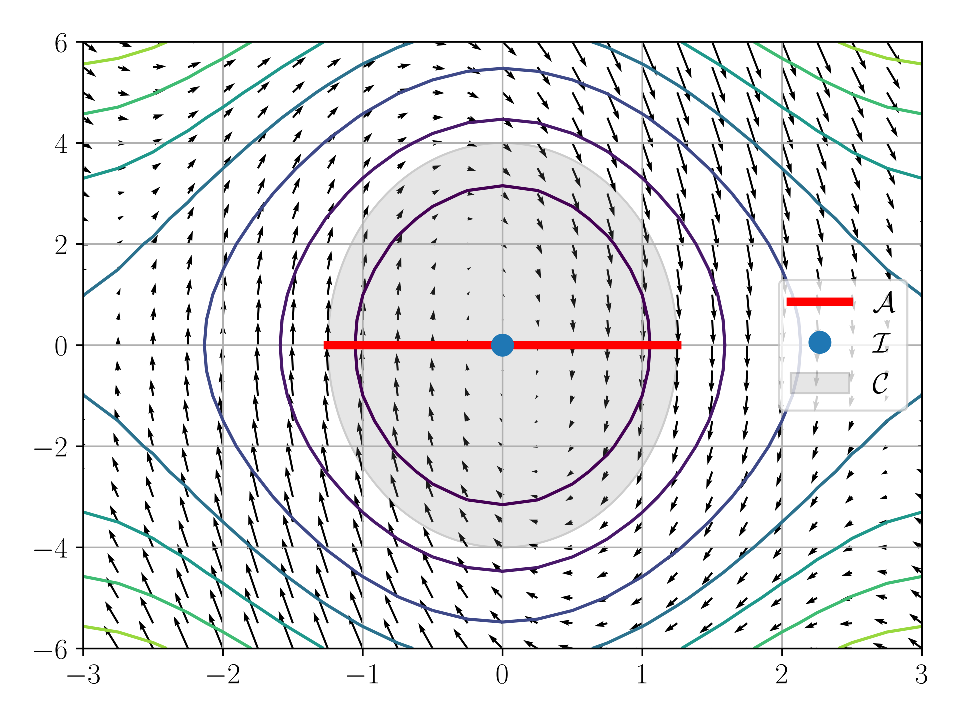
\includegraphics[width=.85\columnwidth]{pendulum.eps}
		\begin{equation*}
			\begin{aligned}
				V(x_1, x_2) = &m g l(1-\cos{x_1}) + \frac{1}{2}\, m l^2 x_2^2
			\end{aligned}
		\end{equation*}
	\end{column}
		
		
	\end{columns}
\end{frame}

\begin{frame}
	\begin{proposition}
		Let  $S : \mathcal{X} \rightarrow R_+$ be a $C^1$ storage
		function for $\Sigma$. Assume that $s$ satisfies
		\begin{equation*}
			s(0, y) \le 0, \qquad \forall y \in Y
		\end{equation*}
		Assume that $x^* \in \mathcal{X}$ is a strict local minimum for $S$. Assume also that no
		solution of $\dot{x} = f (x, 0)$ other than $x(t) \equiv x^∗$ remains in $\{x \in \mathcal{X} |\; s(0, h(x, 0)) = 0\}, \; \forall t$. Then $x^*$ is an asymptotically stable equilibrium of $\dot{x} = f (x, 0)$, which is 	globally asymptotically stable if $V(x):= S(x) - S(x^*) \ge 0$ is proper.
	\end{proposition}
	\textbf{Proof}  $\dot{S}(x) = 0 \implies s(0, h(x, 0)) = 0$. The statement now directly follows from LaSalle’s Invariance
	principle.
	
\end{frame}


\section{Interconnections of dissipative systems}

\begin{frame}{The open character of dissipativity theory}
	Consider $k$ systems $\Sigma_i$  with input, state, and output spaces
	$U_i ,\, \mathcal{X}_i,\, Y_i,\,  i = 1, \dots, k$. Suppose $\Sigma_i$ are dissipative with respect to the supply rates 
	$$s_i(u_i ,y_i), \qquad u_i \in U_i, \; y_i \in Y_i,\;  i = 1, \dots, k,$$
	and storage functions $S_i(x_i), i = 1, \dots, k.$ \\
	Now consider an interconnection of $\Sigma_i, i = 1, \dots, k$, defined through
	\begin{equation*}
		I \subset U_1 \times Y_1 \times \dots \times U_k \times Y_k \times U_e \times Y_e,
	\end{equation*}
	where $U_e , Y_e$ are spaces of external input and output. 
	\begin{proposition}
		Suppose the supply rates $s_1, \dots, s_k$ and the interconnection subset $I$ are such that $\exists s_e : U_e \times Y_e \rightarrow \bbR$ for which
		\begin{equation*}
			\begin{aligned}
				s_1 (u_1, y_1) + \dots + s_k(u_k , y_k) \le s_e(u_e ,y_e), \\
				\forall ((u_1 , y_1 ), \dots, (u_k , y_k), (u_e , y_e)) \in I.
			\end{aligned}
		\end{equation*}
		Then the interconnected system $\Sigma_I$ is dissipative with respect to the supply rate $s_e$,
		with storage function $S(x_1 ,\dots, x_k) := S_1(x_1) + \dots + S_k(x_k)$
	\end{proposition}
	

\end{frame}

\begin{frame}{The Lyapunov function of interconnectd systems}
	
	For simplicity the spaces of external inputs and outputs are removed.	
	\begin{proposition}
		Suppose the supply rates $s_1, \dots, s_k$ and the interconnection subset $I$ are such that there exist positive constants $\alpha_1, \dots, \alpha_k$ for which
		\begin{equation}\label{eq:int_supply}
			\begin{aligned}
				\alpha_1 s_1 (u_1, y_1) + \dots + \alpha_k s_k(u_k , y_k) \le 0, \\
				\forall ((u_1 , y_1 ), \dots, (u_k , y_k)) \in I.
			\end{aligned}
		\end{equation}
	Then the function
	\begin{equation*}
		S_\alpha(x_1 , \dots, x_k) := \alpha_1 S_1(x_1) + \dots + \alpha^k S_k(x_k)
	\end{equation*}
	satisfies $\dot{S}_\alpha \le 0$ along all solutions of the interconnected system $\Sigma_I$.
	\end{proposition}
	\textbf{Proof} It suffices to multiply each dissipation inequality by  $\alpha_1$, add them and use the inequality \eqref{eq:int_supply}.
\end{frame}

\section{Conclusions}


\begin{frame}{Conclusions}
	
	Some important considerations:
	\begin{itemize}
		\item The definition of a dissipative dynamical system postulates the existence of a
		storage function. The dynamical equations are insufficient to specify the storage function uniquely.
		\item  The storage function satisfies an a priori bound. It is bounded from below by the available storage and from above by the required supply. These bounds possess a variational characterization.
		\item In dissipative systems states for which the storage function attains a local minimum are
		locally stable and the storage function is a suitable Lyapunov function.
		\item Immeadiate extension to interconnected systems: the sum of the
		storage functions of the individual subsystems is a storage function for
		the interconnected system.
	\end{itemize}

	
\end{frame}

\begin{frame}{Bibliography}
	%\bibliographystyle{unsrt}
	\nocite{*}
	\printbibliography
\end{frame}

\appendix



	
\end{document}